\section{Appendici}

\begin{frame}
\frametitle{ConvNeXt more benchmark}
Reexamine the design space and push the limits of ConvNet potential, modernizing  standard ResNet towards a Transformer-like design.
This modela have been pretrained on ImageNet-22K pre-trained models.


% \begin{figure}[h]
%     \centering
%     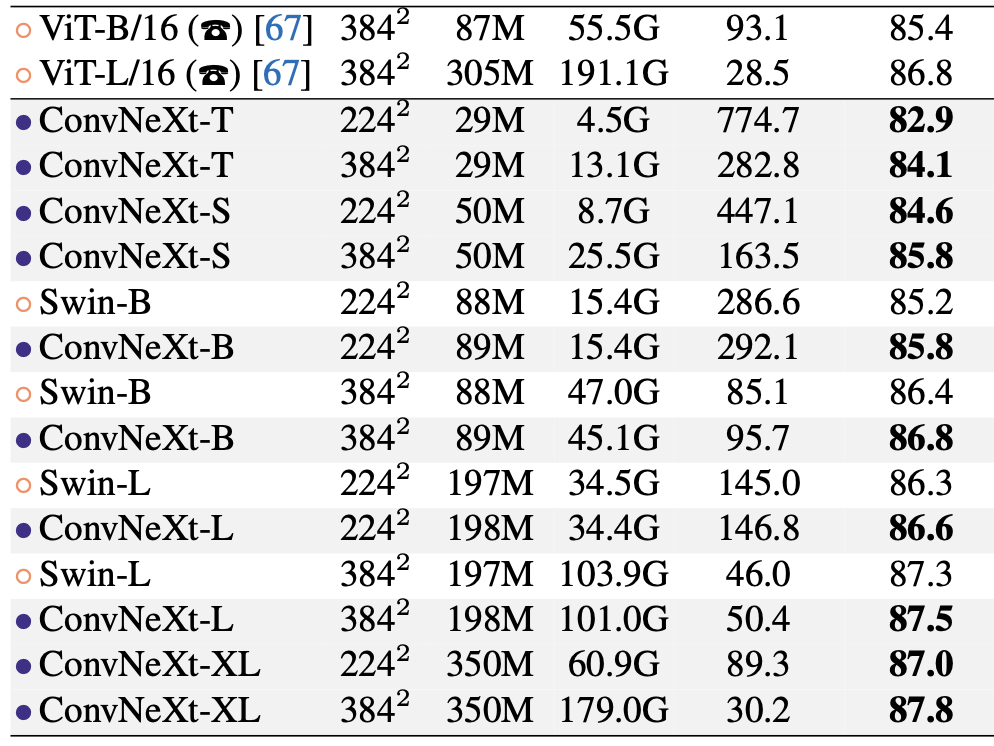
\includegraphics[width=0.7\textwidth]{img/4-section/ConvNext2.png}
%     \caption{Image site, #param, flops, image/s, Tip 1}
% \end{figure}

% \end{frame}


\begin{frame}
\frametitle{More Benchmark with ResNet}
Benchmark between ResNet and ConvNeXt
\begin{center}
    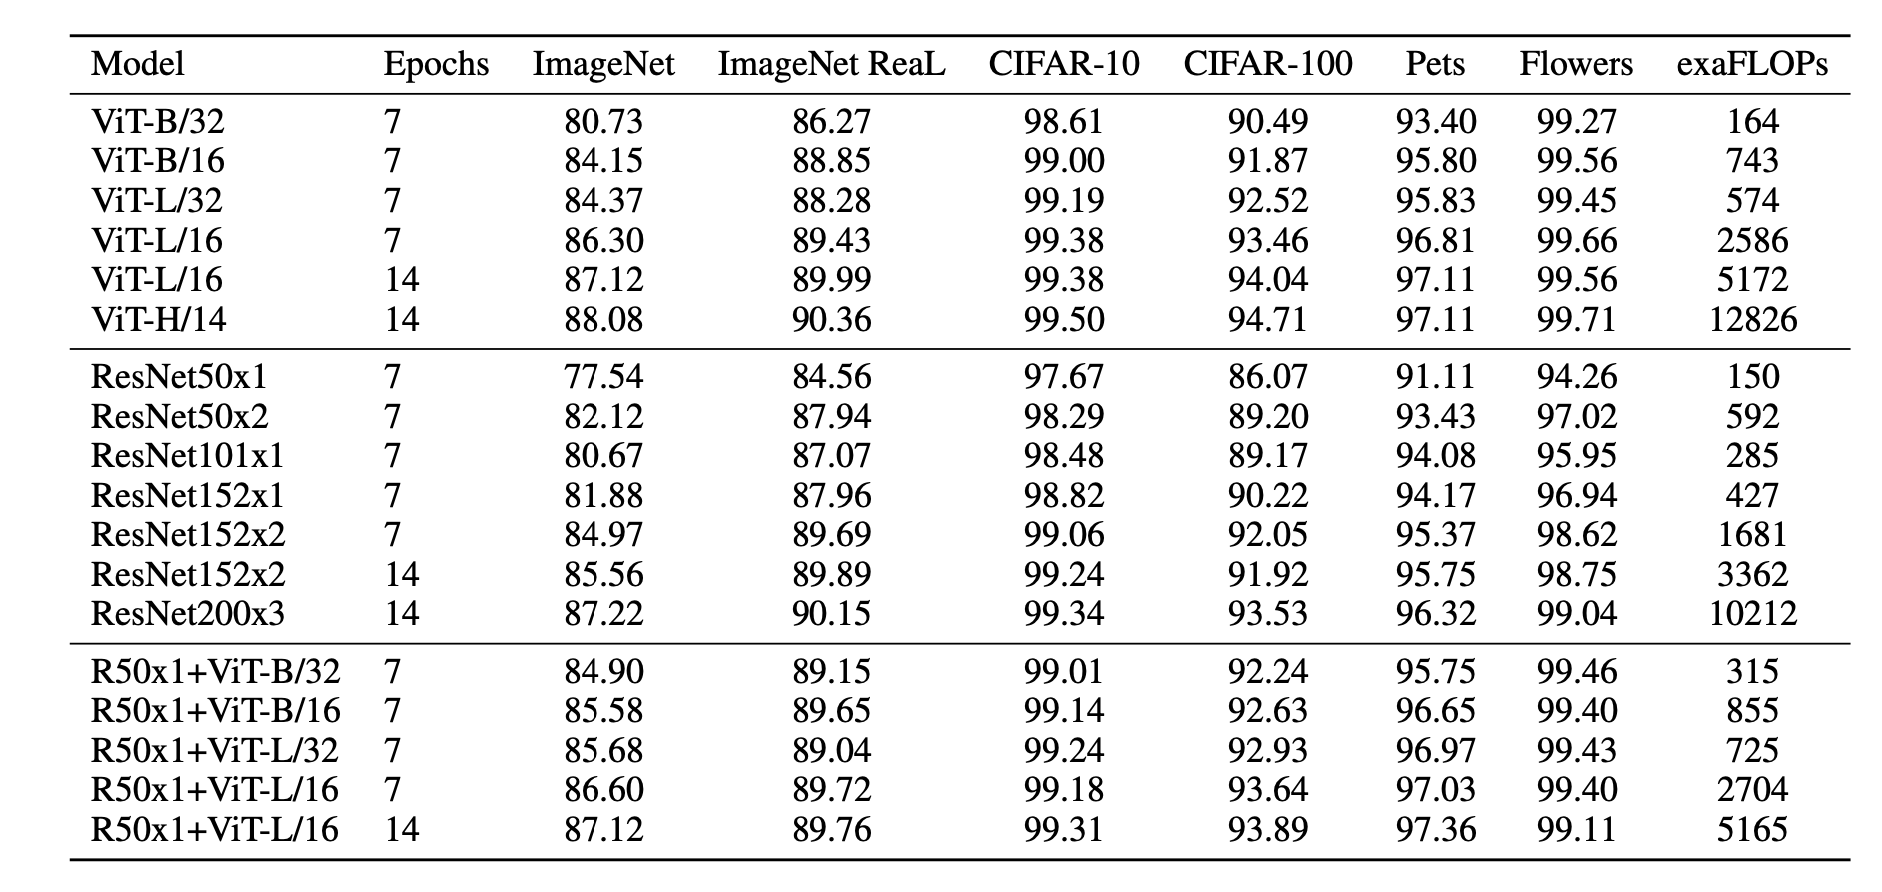
\includegraphics[width=0.7\textwidth]{img/4-section/More-benchmark.png}
\end{center}

\end{frame}

\begin{frame}
\frametitle{Different ViT models}
Benchmark between different ViT models
\begin{center}
    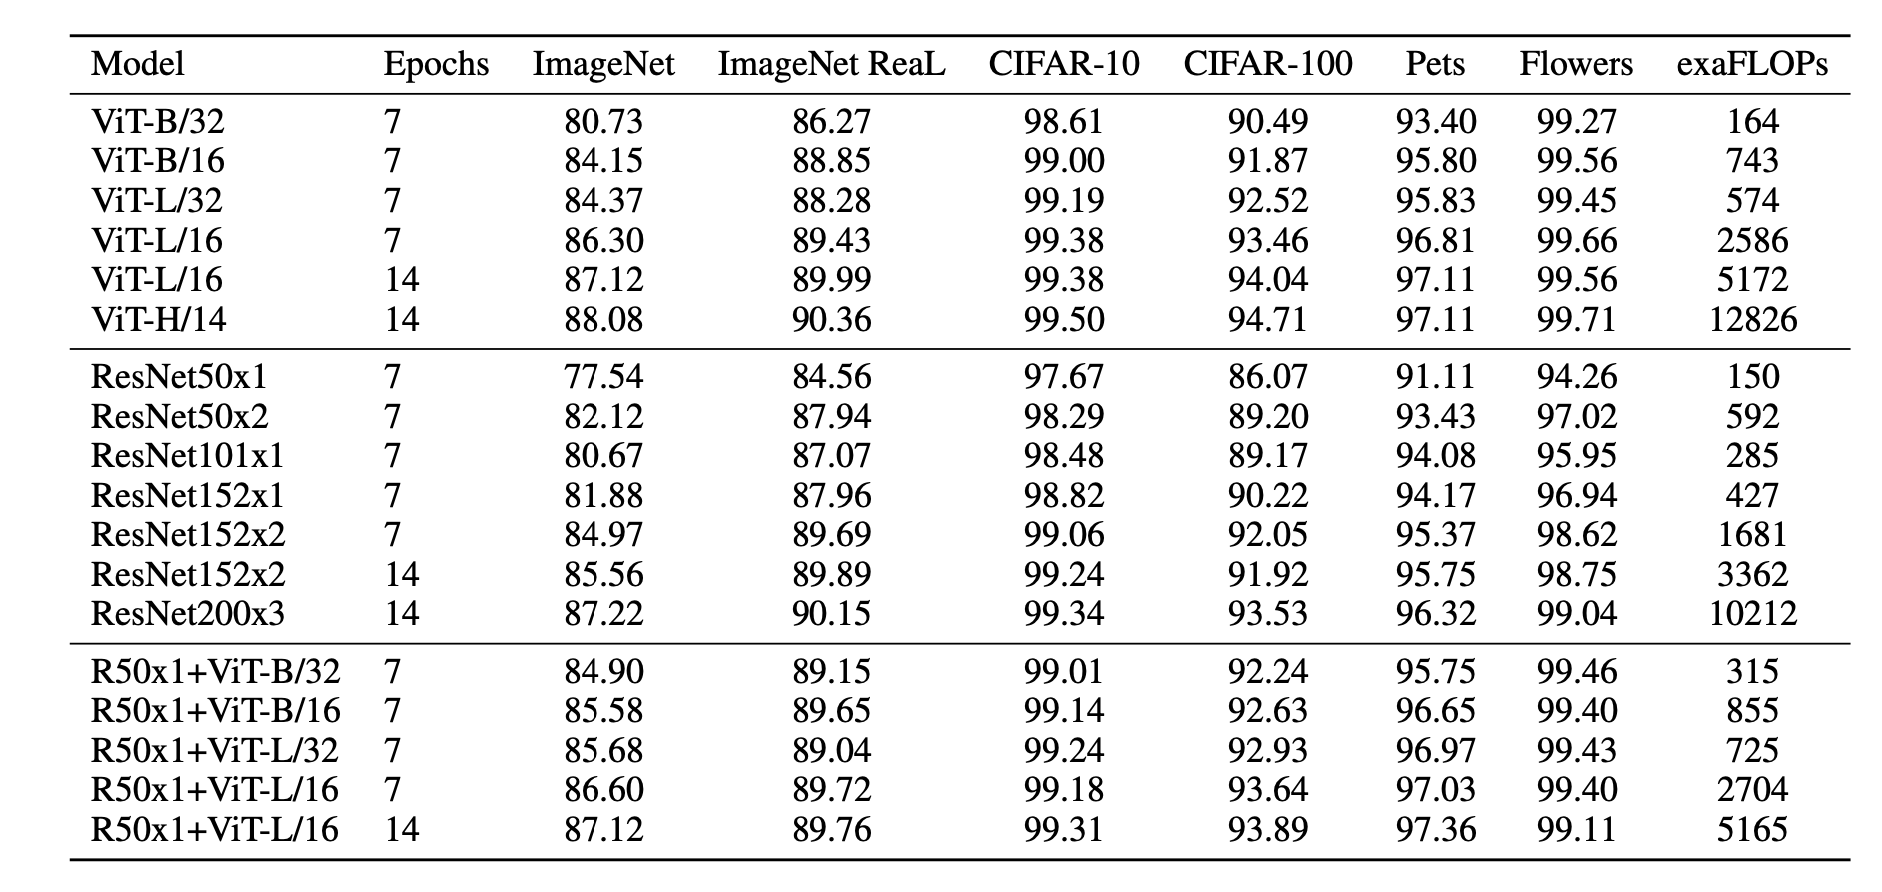
\includegraphics[width=0.7\textwidth]{img/4-section/More-benchmark.png}
\end{center}

\end{frame}


\begin{frame}
\frametitle{Current top 3 Image Classification on ImageNet 1k}
Data has been acquired by the popular \href{https://paperswithcode.com/sota/image-classification-on-imagenet?tag_filter=171}{Papers with Code} website.


\begin{itemize}
    \item \textbf{1st place:} \textit{PeCo} with 88.3\% top-1 accuracy (ViT-H)
    \item \textbf{2nd place:} \textit{MAE} with 87.8\% top-1 accuracy (ViT-H)
    \item \textbf{3rd place:} \textit{PeCo} with 87.5\% top-1 accuracy (ViT-H)
\end{itemize}

\end{frame}

\begin{frame}
\frametitle{Current top 3 Image Classification on ImageNet 22k}
Data has been acquired by the popular \href{https://paperswithcode.com/sota/image-classification-on-imagenet}{Papers with Code} website.


\begin{itemize}
    \item \textbf{1st place:} \textit{OmniVec} 92.4\% accuracy (ViT)
    \item \textbf{1st place:} \textit{BASIC-L} 91.1\% accuracy (ViT)
    \item \textbf{1st place:} \textit{CoCa} 91.0\% accuracy (Multimodal with a ViT)
\end{itemize}

Best ResNet still below 90\% accuracy, best RevCol-H RevCol-H 90.0\% accuracy.

\end{frame}